\chapter{Interaction between fluid flow and elastic obstacle}

\modinfo{Directory}{FsiObstacleGUI}
\modinfo{Solvers}{\Idx{FlowSolve},\Idx{ElasticSolve},\Idx{MeshSolve}}
\modinfo{Tools}{\Idx{ElmerGUI}}
\modinfo{Dimensions}{2D, Steady-state}
\modinfo{Author}{Peter R{\aa}back}


\subsection*{Case definition}
 
%\begin{flushleft}

This tutorial demonstrates how to set up a coupled case
of fluid-structure interaction. Flow is 
initiated at one end of a channel which has an elastic obstacle
that bends under the influence of fluid forces. The resulting displacements 
modify the domain thereby affecting the flow of the fluid.



The channel is assumed to be 2D. The length of the channel is 10~m and the height 
is 2~m. At the distance of 2~m from the inlet sits an elastic beam with a rounded top the height of which is
1.2~m and width 0.4~m. A parabolic velocity profile with maximum velocity
of 1~m/s is assumed.  

Material properties are assumed to be rather simple:
For the structure the density is 
1000~kg/m$^3$, Young's modulus is $1000$~Pa, and Poisson ratio~0.3. For the 
fluid the density is 1~kg/m$^3$ and viscosity is 0.1~Pas. Additionally the 
fluid has elastic properties that are used to extend the displacement 
of the elastic beam to the fluid. 

The idea of the case definition is to 
demonstrate simple yet strongly coupled FSI case without getting into turbulence modelling. Realistic 
material parameters for the given size of the domain would easily result to turbulence and just small 
displacements.

The case is solved using standard weak coupling with some relaxation to
boost the convergence. The solution is steady-state so 
only the final results are will be studied. 

%of thermal flow in curved pipe with a finite thickness. Within the pipe 
%both the flow and heat transfer equations need to be solved while on the
%solid section only heat transfer needs to be considered. 


\subsection*{Solution procedure}


The non-linear elasticity equation is not by default active in the menu structures ElmerGUI. 
Hence, the user must load these before starting the simulations.
\ttbegin
File 
  Definitions
    Append -> nonlinearelastity.xml
\ttend
The additional definitions should reside in the directory \texttt{edf-extra} within the distribution.
Moving the desired \texttt{xml} files to the \texttt{edf}-directory enables automatic loading of the 
definitions at start-up. By inspecting the definitions in the \texttt{Elmer Definitions File editor} one
may inspect that the new definitions were really appended. 


The mesh is defined in .in2d format, the 2D format of 
netgen, in file \texttt{obstacle\_in\_channel.in2d}, load this file.
\ttbegin
File 
  Open -> obstacle\_in\_channel.in2d
\ttend
The default mesh is obviously too sparse. To make the mesh 
more dense set
\ttbegin
Mesh -> Configure -> nglib -> Max H: 0.1 
\ttend
and choose
\ttbegin
Mesh -> Remesh 
\ttend
You should obtain a denser mesh and may check \texttt{Model Summary...} that it consists 
of around 4140 nodes and 7890 linear triangles.

\begin{figure}[h]
\centering
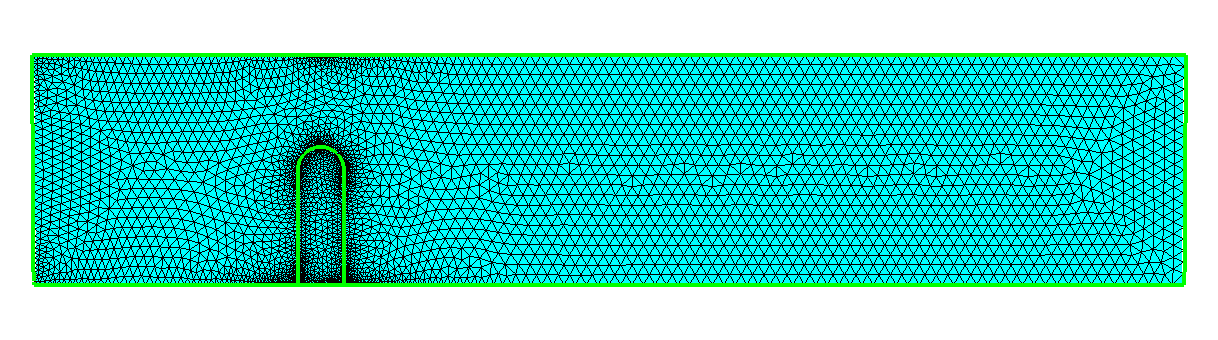
\includegraphics[width=140mm]{fsi_obstacle_gui}
\caption{The mesh of the obstacle in channel case as seen in ElmerGUI}\label{fg:obstacle_in_channel_mesh}
\end{figure} 


After we have the mesh we start to go through the \texttt{Model} menu from the top to bottom. 
In the \texttt{Setup} we choose things related to the whole simulation such as file names, 
time stepping, constants etc.
The simulation is carried out in 2-dimensional Cartesian
coordinates in steady-state. There is not much to do here, just increase the number of iterations needed 
for the convergence of the coupled system. We also set the output interval to zero which means that results are 
written only at the end of the case.
\ttbegin
Model
  Setup 
    Coordinate system = Cartesian
    Simulation type = Steady state
    Steady state max. iter = 100
    Output Intervals = 0
    ...
\ttend

In the Equation section we choose the relevant equations and parameters related to their solution. 
In this case we'll have two different sets of solvers (called as Equation in Elmer slang). 
The fluid domain consists of flow and mesh deformation solvers, while the 
elastic domain just includes the non-linear elasticity solver. We'll name them appropriately. 

To enhance the convergence and efficient use of resources 
we set relaxation factors of the primary solvers to~0.5 and the 
number of non-linear iterations to 1. The mesh deformation solver just extends the 
displacements of the elasticity solver to the fluid domain, so no relaxation is needed here. 
For the linear systems we are quite happy with the defaults.

To honor the causality the flow solver should be solved first, then the elasticity solver and
at last the mesh deformation solver. We set the priorities accordingly. 
\\
\noindent
The equation for the fluid flow + mesh deformation
\ttbegin
Model
  Equation
    Add
    Name = Flow and mesh deform
    Apply to Bodies = 1
    Navier-Stokes
      Active = on
      Priority = 2 
      Edit Solver Setting
        Nonlinear System
          Max.iterations = 1
          Nonlinear System Relaxation Factor = 0.5
    Mesh Update
      Active = on
      Priority = 0 
    OK
\ttend        
and then for the solid
\ttbegin
Model
  Equation
    Add
    Name = Elasticty
    Apply to Bodies = 2
    Nonlinear Elasticty
      Active = on
      Priority = 1
      Edit Solver Setting
        Nonlinear System
          Max.iterations = 1
          Nonlinear System Relaxation Factor = 0.5
    OK
\ttend    

Next we set our rather simple material parameters.
The Material section includes all the material parameters.
They are divided into generic parameters which are direct properties of the material
without making any assumptions on the physical model, such as the density. Other properties assume
a physical law, such as conductivities and viscosity. 

\ttbegin
Model
  Material
    Add
    Name = Ideal fluid 
    General 
      Density = 1.0
    Navier-Stokes
      Viscosity = 0.1
    Mesh Update
      Elastic Modulus = 1.0
      Poisson Ratio = 0.3  
    Apply to Bodies = 1 
    OK

    Add  
    Name = Ideal structure
    General 
      Density = 1.0e3
    Nonlinear Elasticity
      Youngs Modulus = 1.0e3
      Poisson Ratio = 0.3
    Apply to Bodies = 2
    OK
\ttend

The \texttt{Body force} section usually represents the right-hand-side of an equation. 
In this case we do not need any body forces.

Also an \texttt{Initial condition} could be given in steady-state case to enhance convergence. However, 
in this case convergence is pretty robust with the default guess of zero.

We have five different boundary conditions: inflow, outflow, lateral walls with no-slip conditions, 
fsi conditions, and the beam base. 
As it is tedious to know the indexes by heart we 
first define the different BCs and only afterwards apply them to the existing boundaries 
with the mouse. 

\ttbegin
Model
  BoundaryCondition
    Name = Inflow
    Navier-Stokes 
      Velocity 1 = Variable Coordinate 2 
        Real MATC "tx*(2-tx)"
      Velocity 2 = 0.0
      Mesh Update 1 = 0.0
    Add
    New
\ttend
The condition for \texttt{Velocity 1} above may easiest be typed by pressing \texttt{Enter}-key in the
edit box which will open a larger window for editing.
\ttbegin
    Name = Outflow
    Navier-Stokes 
      Velocity 2 = 0.0
    Mesh Update
      Mesh Update 1 = 0.0
    Add
    New

    Name = Walls
    Navier-Stokes 
      NoSlip Wall BC = on
    Mesh Update
      Mesh Update 1 = 0.0
      Mesh Update 2 = 0.0
    Add 
    New
 
    Name = Base
    Nonlinear Elasticity
      Displacement 1 = 0.0
      Displacement 2 = 0.0
    Add
    New
\ttend
The essence of fluid-structure interaction is in the following boundary condition. 
When the \texttt{Fsi BC} is active the fluid forces are automatically within ElasticSolver.
The back coupling to Navier-Stokes is achieved through the change in fluid geometry which is enforced
by the conditions for the \texttt{MeshSolver}.
\ttbegin
    Name = FSI 
    Nonlinear Elasticity 
      FSI BC = on
    Navier-Stokes 
      NoSlip Wall BC = on
    Mesh Update 1 = Equals Displacement 1
    Mesh Update 2 = Equals Displacement 2
\ttend   

Now we are ready to choose the boundaries 
\ttbegin
Model
  Set boundary properties
    Choose inlet side -> set boundary condition Inflow
    Choose outlet side -> set boundary condition Outflow
    Choose upper and lower sides (three pieces) -> set boundary condition Walls
    Choose obstacle base -> set boundary condition Base
    Choose interface between fluid and solid (two pieces) -> set boundary condition FSI
\ttend

For the execution 
ElmerSolver needs the mesh files and the command file. We have now basically defined
all the information for ElmerGUI to write the command file. After writing it we may also visually 
inspect the command file.
\ttbegin
Sif 
  Generate
  Edit -> look how your command file came out  
\ttend

Before we can execute the solver we should save the files in a directory. The project includes
all the files needed to restart the case. It's a good idea to give the project an illuminating name.
Avoid paths which includes empty spaces since they may cause problems later on. 
\ttbegin
File 
  Save Project
    Make New Folder -> fsi_obstacle
    OK
\ttend

After we have successfully saved the files we may start the solver
\ttbegin
Run
  Start solver
\ttend
A convergence view automatically pops up showing relative changes of each iteration.
The simulation may take around ~10 seconds depending on your platform. 

The computed norms should be around 0.514 for the Navier-Stokes solver, 0.108 for the elasticity solver,
and 0.0548 for the mesh update solver. These are reached after 18 iterations using the rather strict default settings.

If there is some discrepancy the setup of the system
was probably different from the one in the tutorial.
If the results are in agreement we are ready to look at the results.

\subsection*{Results}

To visualize the results open the postprocessor, in this case \texttt{ParaView}
After the simulation has terminated we may open the postprocessor to view the results.
\ttbegin
Run
  Start ParaView
\ttend

For flow problems we can visualize pressure (or velocity amplitudes) separately with the vector presentation
of the velocity field. In Paraview the filter to apply the displacement field to the nodal coordinates is
called \texttt{WarpByVector}.

The maximum speed in the system is around 2.328 and the maximum displacement 0.2636. Note that 
for the saved results the displacement and mesh update fields have been merged into one. 
In Figures \ref{fg:fsi_obstacle_velo}, \ref{fg:fsi_obstacle_pres}, and
\ref{fg:fsi_obstacle_disp}
the obtained velocity, pressure and displacement 
distributions are presented in the deformed mesh.  A close up showing the deformed mesh is shown
in figure  \ref{fg:fsi_obstacle_deformed}
 
\begin{figure}[h]
\centering
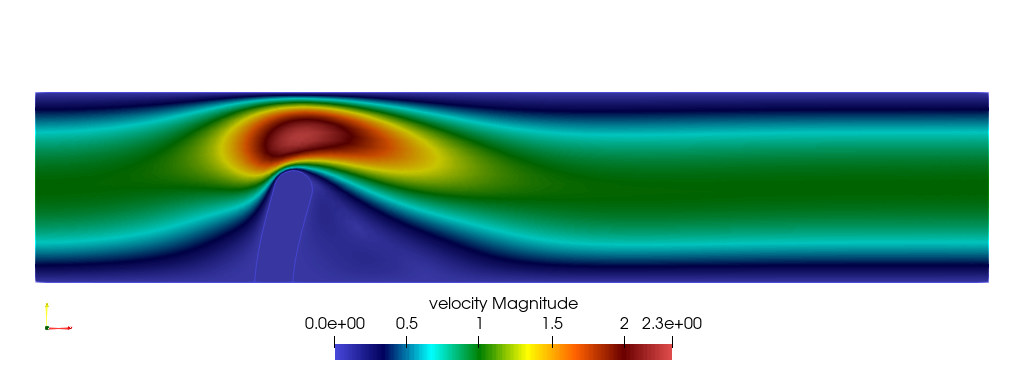
\includegraphics[width=140mm,viewport=0 5 1024 400,clip]{fsi_obstacle_velo}
\caption{Velocity distribution of the obstacle in channel case.}\label{fg:fsi_obstacle_velo}
\end{figure} 

\begin{figure}[h]
\centering
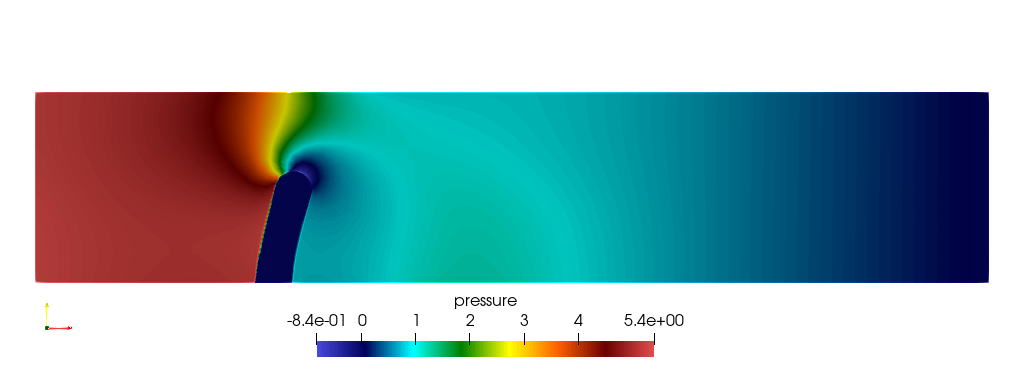
\includegraphics[width=140mm,viewport=0 5 1024 400,clip]{fsi_obstacle_pres}
\caption{Pressure distribution of the obstacle in channel case.}\label{fg:fsi_obstacle_pres}
\end{figure} 

\begin{figure}[h]
\centering
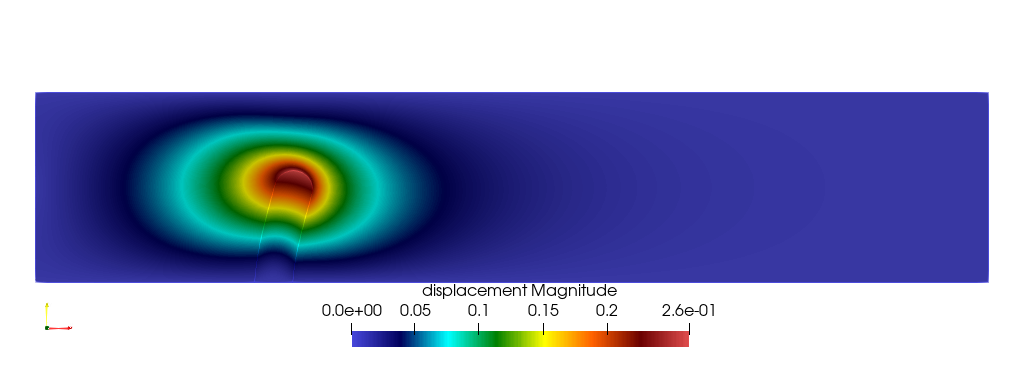
\includegraphics[width=140mm,viewport=0 5 1024 400,clip]{fsi_obstacle_disp}
\caption{Displacement distribution of the obstacle in channel case.}\label{fg:fsi_obstacle_disp}
\end{figure} 

\begin{figure}[h]
\centering
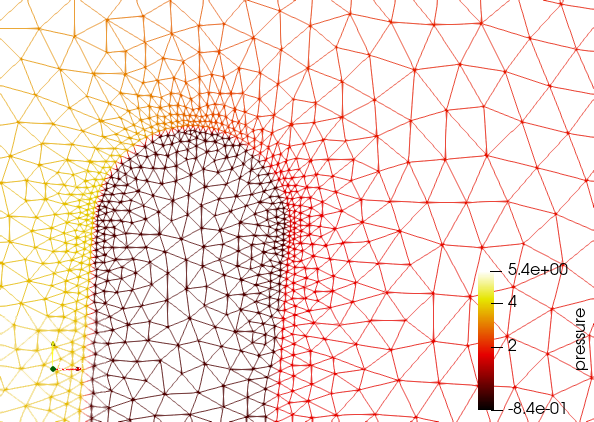
\includegraphics[width=140mm]{fsi_obstacle_deformed}
\caption{Deformed mesh of the obstacle in channel case.}\label{fg:fsi_obstacle_deformed}
\end{figure} 



\hfill
\mbox{}
